% Created by tikzDevice version 0.12.5 on 2023-10-05 23:41:38
% !TEX encoding = UTF-8 Unicode
\definecolor{triplet}{HTML}{E69F00}
\definecolor{mar-sum}{HTML}{009E73}
\definecolor{mar-max}{HTML}{CC79A7}
\definecolor{color1}{HTML}{CC9966}
\definecolor{color2}{HTML}{99CCFF}
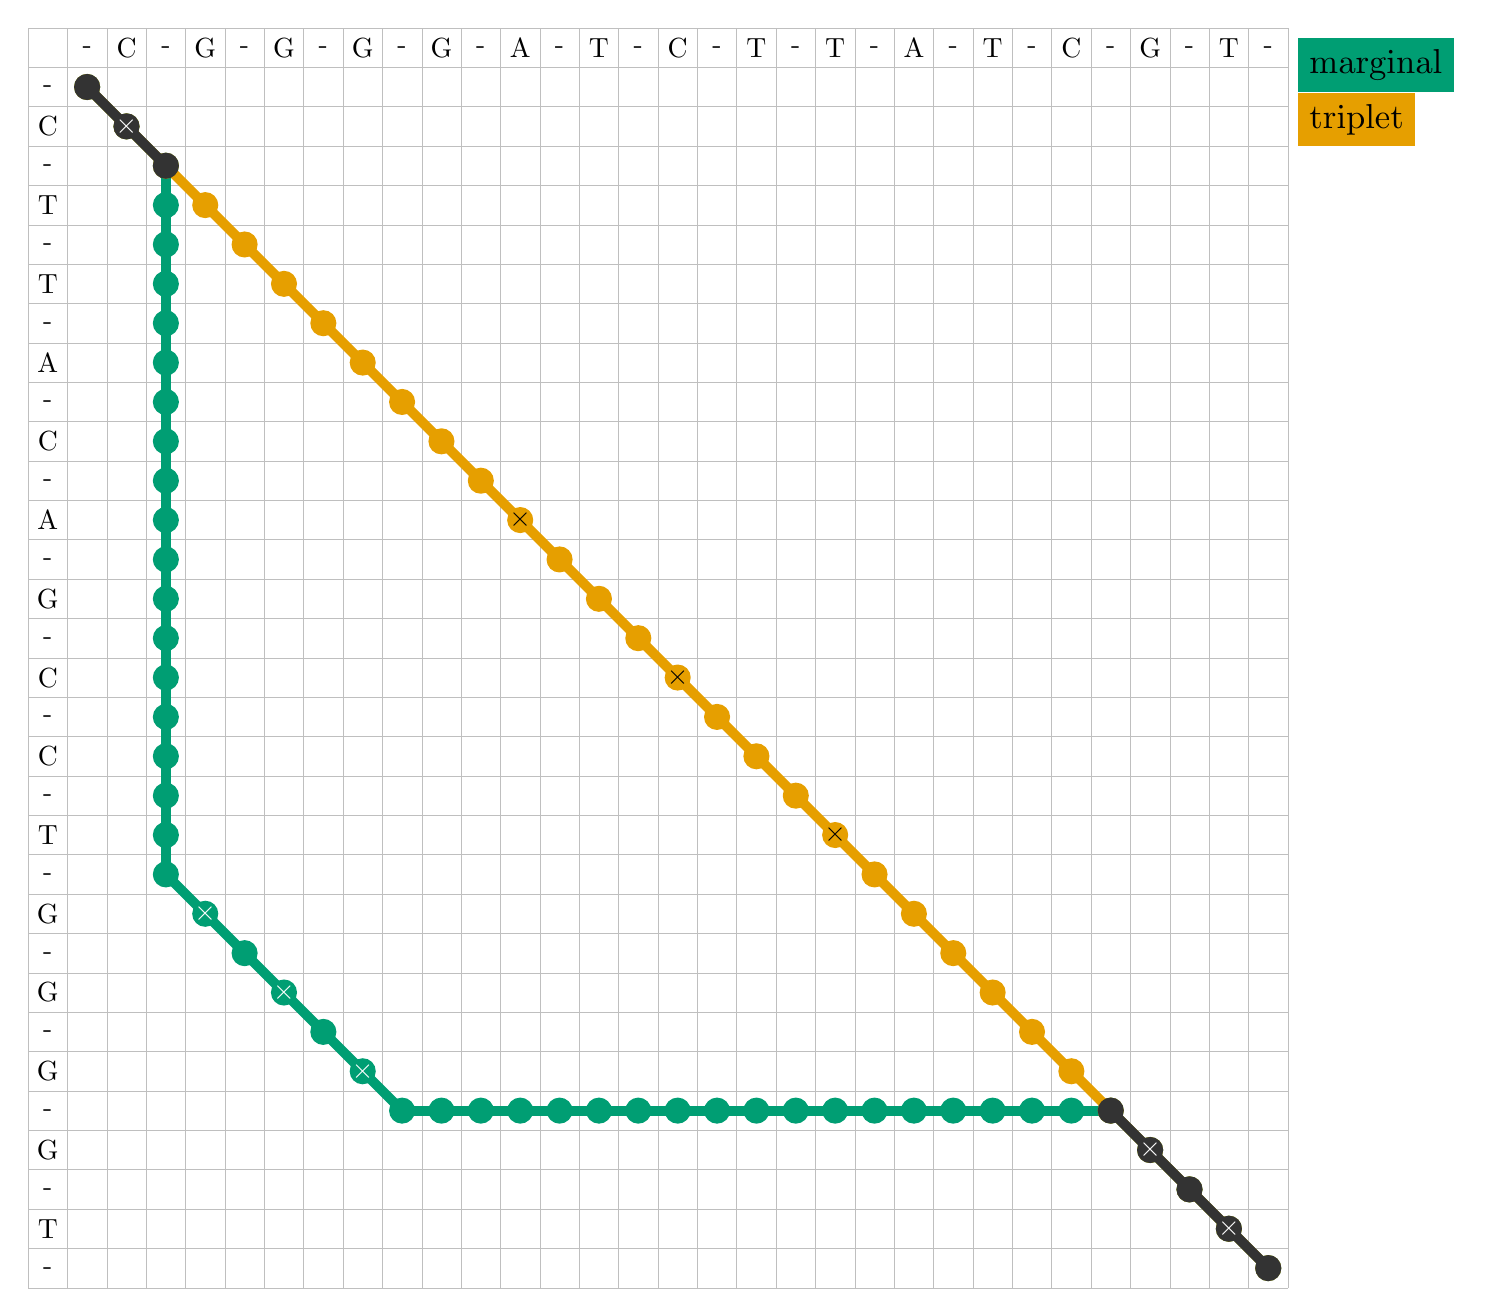
\begin{tikzpicture}[dot/.style={circle, minimum size=2.5mm}, box/.style={rectangle, minimum size = 3.5cm, anchor = north west}]
\draw[very thin, color = gray!50, step = 0.5] (0,0) grid (16, 16);
\node at (0.25,15.25) {-};
\node at (0.25,14.75) {C};
\node at (0.25,14.25) {-};
\node at (0.25,13.75) {T};
\node at (0.25,13.25) {-};
\node at (0.25,12.75) {T};
\node at (0.25,12.25) {-};
\node at (0.25,11.75) {A};
\node at (0.25,11.25) {-};
\node at (0.25,10.75) {C};
\node at (0.25,10.25) {-};
\node at (0.25,9.75) {A};
\node at (0.25,9.25) {-};
\node at (0.25,8.75) {G};
\node at (0.25,8.25) {-};
\node at (0.25,7.75) {C};
\node at (0.25,7.25) {-};
\node at (0.25,6.75) {C};
\node at (0.25,6.25) {-};
\node at (0.25,5.75) {T};
\node at (0.25,5.25) {-};
\node at (0.25,4.75) {G};
\node at (0.25,4.25) {-};
\node at (0.25,3.75) {G};
\node at (0.25,3.25) {-};
\node at (0.25,2.75) {G};
\node at (0.25,2.25) {-};
\node at (0.25,1.75) {G};
\node at (0.25,1.25) {-};
\node at (0.25,0.75) {T};
\node at (0.25,0.25) {-};
\node at (0.75,15.75) {-};
\node at (1.25,15.75) {C};
\node at (1.75,15.75) {-};
\node at (2.25,15.75) {G};
\node at (2.75,15.75) {-};
\node at (3.25,15.75) {G};
\node at (3.75,15.75) {-};
\node at (4.25,15.75) {G};
\node at (4.75,15.75) {-};
\node at (5.25,15.75) {G};
\node at (5.75,15.75) {-};
\node at (6.25,15.75) {A};
\node at (6.75,15.75) {-};
\node at (7.25,15.75) {T};
\node at (7.75,15.75) {-};
\node at (8.25,15.75) {C};
\node at (8.75,15.75) {-};
\node at (9.25,15.75) {T};
\node at (9.75,15.75) {-};
\node at (10.25,15.75) {T};
\node at (10.75,15.75) {-};
\node at (11.25,15.75) {A};
\node at (11.75,15.75) {-};
\node at (12.25,15.75) {T};
\node at (12.75,15.75) {-};
\node at (13.25,15.75) {C};
\node at (13.75,15.75) {-};
\node at (14.25,15.75) {G};
\node at (14.75,15.75) {-};
\node at (15.25,15.75) {T};
\node at (15.75,15.75) {-};
\draw[line width=1.25mm,mar-sum](0.75,15.25)--(1.25,14.75);
\node[circle, fill=mar-sum] at (0.75, 15.25){};
\draw[line width=1.25mm,mar-sum](1.25,14.75)--(1.75,14.25);
\node[circle, fill=mar-sum] at (1.25, 14.75){};
\node[white] at (1.25, 14.75){$\mathlarger{\mathlarger{\bm{\times}}}$};
\draw[line width=1.25mm,mar-sum](1.75,14.25)--(1.75,13.75);
\node[circle, fill=mar-sum] at (1.75, 14.25){};
\draw[line width=1.25mm,mar-sum](1.75,13.75)--(1.75,13.25);
\node[circle, fill=mar-sum] at (1.75, 13.75){};
\draw[line width=1.25mm,mar-sum](1.75,13.25)--(1.75,12.75);
\node[circle, fill=mar-sum] at (1.75, 13.25){};
\draw[line width=1.25mm,mar-sum](1.75,12.75)--(1.75,12.25);
\node[circle, fill=mar-sum] at (1.75, 12.75){};
\draw[line width=1.25mm,mar-sum](1.75,12.25)--(1.75,11.75);
\node[circle, fill=mar-sum] at (1.75, 12.25){};
\draw[line width=1.25mm,mar-sum](1.75,11.75)--(1.75,11.25);
\node[circle, fill=mar-sum] at (1.75, 11.75){};
\draw[line width=1.25mm,mar-sum](1.75,11.25)--(1.75,10.75);
\node[circle, fill=mar-sum] at (1.75, 11.25){};
\draw[line width=1.25mm,mar-sum](1.75,10.75)--(1.75,10.25);
\node[circle, fill=mar-sum] at (1.75, 10.75){};
\draw[line width=1.25mm,mar-sum](1.75,10.25)--(1.75,9.75);
\node[circle, fill=mar-sum] at (1.75, 10.25){};
\draw[line width=1.25mm,mar-sum](1.75,9.75)--(1.75,9.25);
\node[circle, fill=mar-sum] at (1.75, 9.75){};
\draw[line width=1.25mm,mar-sum](1.75,9.25)--(1.75,8.75);
\node[circle, fill=mar-sum] at (1.75, 9.25){};
\draw[line width=1.25mm,mar-sum](1.75,8.75)--(1.75,8.25);
\node[circle, fill=mar-sum] at (1.75, 8.75){};
\draw[line width=1.25mm,mar-sum](1.75,8.25)--(1.75,7.75);
\node[circle, fill=mar-sum] at (1.75, 8.25){};
\draw[line width=1.25mm,mar-sum](1.75,7.75)--(1.75,7.25);
\node[circle, fill=mar-sum] at (1.75, 7.75){};
\draw[line width=1.25mm,mar-sum](1.75,7.25)--(1.75,6.75);
\node[circle, fill=mar-sum] at (1.75, 7.25){};
\draw[line width=1.25mm,mar-sum](1.75,6.75)--(1.75,6.25);
\node[circle, fill=mar-sum] at (1.75, 6.75){};
\draw[line width=1.25mm,mar-sum](1.75,6.25)--(1.75,5.75);
\node[circle, fill=mar-sum] at (1.75, 6.25){};
\draw[line width=1.25mm,mar-sum](1.75,5.75)--(1.75,5.25);
\node[circle, fill=mar-sum] at (1.75, 5.75){};
\draw[line width=1.25mm,mar-sum](1.75,5.25)--(2.25,4.75);
\node[circle, fill=mar-sum] at (1.75, 5.25){};
\draw[line width=1.25mm,mar-sum](2.25,4.75)--(2.75,4.25);
\node[circle, fill=mar-sum] at (2.25, 4.75){};
\node[white] at (2.25, 4.75){$\mathlarger{\mathlarger{\bm{\times}}}$};
\draw[line width=1.25mm,mar-sum](2.75,4.25)--(3.25,3.75);
\node[circle, fill=mar-sum] at (2.75, 4.25){};
\draw[line width=1.25mm,mar-sum](3.25,3.75)--(3.75,3.25);
\node[circle, fill=mar-sum] at (3.25, 3.75){};
\node[white] at (3.25, 3.75){$\mathlarger{\mathlarger{\bm{\times}}}$};
\draw[line width=1.25mm,mar-sum](3.75,3.25)--(4.25,2.75);
\node[circle, fill=mar-sum] at (3.75, 3.25){};
\draw[line width=1.25mm,mar-sum](4.25,2.75)--(4.75,2.25);
\node[circle, fill=mar-sum] at (4.25, 2.75){};
\node[white] at (4.25, 2.75){$\mathlarger{\mathlarger{\bm{\times}}}$};
\draw[line width=1.25mm,mar-sum](4.75,2.25)--(5.25,2.25);
\node[circle, fill=mar-sum] at (4.75, 2.25){};
\draw[line width=1.25mm,mar-sum](5.25,2.25)--(5.75,2.25);
\node[circle, fill=mar-sum] at (5.25, 2.25){};
\draw[line width=1.25mm,mar-sum](5.75,2.25)--(6.25,2.25);
\node[circle, fill=mar-sum] at (5.75, 2.25){};
\draw[line width=1.25mm,mar-sum](6.25,2.25)--(6.75,2.25);
\node[circle, fill=mar-sum] at (6.25, 2.25){};
\draw[line width=1.25mm,mar-sum](6.75,2.25)--(7.25,2.25);
\node[circle, fill=mar-sum] at (6.75, 2.25){};
\draw[line width=1.25mm,mar-sum](7.25,2.25)--(7.75,2.25);
\node[circle, fill=mar-sum] at (7.25, 2.25){};
\draw[line width=1.25mm,mar-sum](7.75,2.25)--(8.25,2.25);
\node[circle, fill=mar-sum] at (7.75, 2.25){};
\draw[line width=1.25mm,mar-sum](8.25,2.25)--(8.75,2.25);
\node[circle, fill=mar-sum] at (8.25, 2.25){};
\draw[line width=1.25mm,mar-sum](8.75,2.25)--(9.25,2.25);
\node[circle, fill=mar-sum] at (8.75, 2.25){};
\draw[line width=1.25mm,mar-sum](9.25,2.25)--(9.75,2.25);
\node[circle, fill=mar-sum] at (9.25, 2.25){};
\draw[line width=1.25mm,mar-sum](9.75,2.25)--(10.25,2.25);
\node[circle, fill=mar-sum] at (9.75, 2.25){};
\draw[line width=1.25mm,mar-sum](10.25,2.25)--(10.75,2.25);
\node[circle, fill=mar-sum] at (10.25, 2.25){};
\draw[line width=1.25mm,mar-sum](10.75,2.25)--(11.25,2.25);
\node[circle, fill=mar-sum] at (10.75, 2.25){};
\draw[line width=1.25mm,mar-sum](11.25,2.25)--(11.75,2.25);
\node[circle, fill=mar-sum] at (11.25, 2.25){};
\draw[line width=1.25mm,mar-sum](11.75,2.25)--(12.25,2.25);
\node[circle, fill=mar-sum] at (11.75, 2.25){};
\draw[line width=1.25mm,mar-sum](12.25,2.25)--(12.75,2.25);
\node[circle, fill=mar-sum] at (12.25, 2.25){};
\draw[line width=1.25mm,mar-sum](12.75,2.25)--(13.25,2.25);
\node[circle, fill=mar-sum] at (12.75, 2.25){};
\draw[line width=1.25mm,mar-sum](13.25,2.25)--(13.75,2.25);
\node[circle, fill=mar-sum] at (13.25, 2.25){};
\draw[line width=1.25mm,mar-sum](13.75,2.25)--(14.25,1.75);
\node[circle, fill=mar-sum] at (13.75, 2.25){};
\draw[line width=1.25mm,mar-sum](14.25,1.75)--(14.75,1.25);
\node[circle, fill=mar-sum] at (14.25, 1.75){};
\node[white] at (14.25, 1.75){$\mathlarger{\mathlarger{\bm{\times}}}$};
\draw[line width=1.25mm,mar-sum](14.75,1.25)--(15.25,0.75);
\node[circle, fill=mar-sum] at (14.75, 1.25){};
\draw[line width=1.25mm,mar-sum](15.25,0.75)--(15.75,0.25);
\node[circle, fill=mar-sum] at (15.25, 0.75){};
\node[white] at (15.25, 0.75){$\mathlarger{\mathlarger{\bm{\times}}}$};
\node[circle, fill=mar-sum] at (15.75, 0.25){};
\draw[line width=1.25mm,triplet](0.75,15.25)--(1.25,14.75);
\node[circle, fill=triplet] at (0.75, 15.25){};
\draw[line width=1.25mm,triplet](1.25,14.75)--(1.75,14.25);
\node[circle, fill=triplet] at (1.25, 14.75){};
\node[black] at (1.25, 14.75){$\mathlarger{\mathlarger{\bm{\times}}}$};
\draw[line width=1.25mm,triplet](1.75,14.25)--(2.25,13.75);
\node[circle, fill=triplet] at (1.75, 14.25){};
\draw[line width=1.25mm,triplet](2.25,13.75)--(2.75,13.25);
\node[circle, fill=triplet] at (2.25, 13.75){};
\draw[line width=1.25mm,triplet](2.75,13.25)--(3.25,12.75);
\node[circle, fill=triplet] at (2.75, 13.25){};
\draw[line width=1.25mm,triplet](3.25,12.75)--(3.75,12.25);
\node[circle, fill=triplet] at (3.25, 12.75){};
\draw[line width=1.25mm,triplet](3.75,12.25)--(4.25,11.75);
\node[circle, fill=triplet] at (3.75, 12.25){};
\draw[line width=1.25mm,triplet](4.25,11.75)--(4.75,11.25);
\node[circle, fill=triplet] at (4.25, 11.75){};
\draw[line width=1.25mm,triplet](4.75,11.25)--(5.25,10.75);
\node[circle, fill=triplet] at (4.75, 11.25){};
\draw[line width=1.25mm,triplet](5.25,10.75)--(5.75,10.25);
\node[circle, fill=triplet] at (5.25, 10.75){};
\draw[line width=1.25mm,triplet](5.75,10.25)--(6.25,9.75);
\node[circle, fill=triplet] at (5.75, 10.25){};
\draw[line width=1.25mm,triplet](6.25,9.75)--(6.75,9.25);
\node[circle, fill=triplet] at (6.25, 9.75){};
\node[black] at (6.25, 9.75){$\mathlarger{\mathlarger{\bm{\times}}}$};
\draw[line width=1.25mm,triplet](6.75,9.25)--(7.25,8.75);
\node[circle, fill=triplet] at (6.75, 9.25){};
\draw[line width=1.25mm,triplet](7.25,8.75)--(7.75,8.25);
\node[circle, fill=triplet] at (7.25, 8.75){};
\draw[line width=1.25mm,triplet](7.75,8.25)--(8.25,7.75);
\node[circle, fill=triplet] at (7.75, 8.25){};
\draw[line width=1.25mm,triplet](8.25,7.75)--(8.75,7.25);
\node[circle, fill=triplet] at (8.25, 7.75){};
\node[black] at (8.25, 7.75){$\mathlarger{\mathlarger{\bm{\times}}}$};
\draw[line width=1.25mm,triplet](8.75,7.25)--(9.25,6.75);
\node[circle, fill=triplet] at (8.75, 7.25){};
\draw[line width=1.25mm,triplet](9.25,6.75)--(9.75,6.25);
\node[circle, fill=triplet] at (9.25, 6.75){};
\draw[line width=1.25mm,triplet](9.75,6.25)--(10.25,5.75);
\node[circle, fill=triplet] at (9.75, 6.25){};
\draw[line width=1.25mm,triplet](10.25,5.75)--(10.75,5.25);
\node[circle, fill=triplet] at (10.25, 5.75){};
\node[black] at (10.25, 5.75){$\mathlarger{\mathlarger{\bm{\times}}}$};
\draw[line width=1.25mm,triplet](10.75,5.25)--(11.25,4.75);
\node[circle, fill=triplet] at (10.75, 5.25){};
\draw[line width=1.25mm,triplet](11.25,4.75)--(11.75,4.25);
\node[circle, fill=triplet] at (11.25, 4.75){};
\draw[line width=1.25mm,triplet](11.75,4.25)--(12.25,3.75);
\node[circle, fill=triplet] at (11.75, 4.25){};
\draw[line width=1.25mm,triplet](12.25,3.75)--(12.75,3.25);
\node[circle, fill=triplet] at (12.25, 3.75){};
\draw[line width=1.25mm,triplet](12.75,3.25)--(13.25,2.75);
\node[circle, fill=triplet] at (12.75, 3.25){};
\draw[line width=1.25mm,triplet](13.25,2.75)--(13.75,2.25);
\node[circle, fill=triplet] at (13.25, 2.75){};
\draw[line width=1.25mm,triplet](13.75,2.25)--(14.25,1.75);
\node[circle, fill=triplet] at (13.75, 2.25){};
\draw[line width=1.25mm,triplet](14.25,1.75)--(14.75,1.25);
\node[circle, fill=triplet] at (14.25, 1.75){};
\node[black] at (14.25, 1.75){$\mathlarger{\mathlarger{\bm{\times}}}$};
\draw[line width=1.25mm,triplet](14.75,1.25)--(15.25,0.75);
\node[circle, fill=triplet] at (14.75, 1.25){};
\draw[line width=1.25mm,triplet](15.25,0.75)--(15.75,0.25);
\node[circle, fill=triplet] at (15.25, 0.75){};
\node[black] at (15.25, 0.75){$\mathlarger{\mathlarger{\bm{\times}}}$};
\node[circle, fill=triplet] at (15.75, 0.25){};
\draw[line width=1.25mm,black!80](0.75,15.25)--(1.25,14.75);
\node[circle, fill=black!80] at (0.75, 15.25){};
\draw[line width=1.25mm,black!80](1.25,14.75)--(1.75,14.25);
\node[circle, fill=black!80] at (1.25, 14.75){};
\node[white] at (1.25, 14.75){$\mathlarger{\mathlarger{\bm{\times}}}$};
\node[circle, fill=black!80] at (1.75, 14.25){};
\draw[line width=1.25mm,black!80](13.75,2.25)--(14.25,1.75);
\node[circle, fill=black!80] at (13.75, 2.25){};
\draw[line width=1.25mm,black!80](14.25,1.75)--(14.75,1.25);
\node[circle, fill=black!80] at (14.25, 1.75){};
\node[white] at (14.25, 1.75){$\mathlarger{\mathlarger{\bm{\times}}}$};
\draw[line width=1.25mm,black!80](14.75,1.25)--(15.25,0.75);
\node[circle, fill=black!80] at (14.75, 1.25){};
\draw[line width=1.25mm,black!80](15.25,0.75)--(15.75,0.25);
\node[circle, fill=black!80] at (15.25, 0.75){};
\node[white] at (15.25, 0.75){$\mathlarger{\mathlarger{\bm{\times}}}$};
\node[circle, fill=black!80] at (15.75, 0.25){};
\matrix [draw, below right, draw=none] at (current bounding box.north east) {
        \node[rectangle, fill=mar-sum, scale=1.25] {marginal}; \\
        \node[rectangle, fill=triplet, scale=1.25] {triplet}; \\
    };
\end{tikzpicture}
